\chapter{Methodologies}
\section{Methodologies}

This chapter presents the machine learning methodologies employed to construct surrogate models for fast and accurate prediction of thermal system behavior. The goal of these models is to approximate the mapping between operating conditions and the reduced latent representation of time-dependent thermal outputs obtained from high-fidelity Dymola simulations. Among the evaluated approaches, ensemble-based and neural network–based regression models are considered. This section first introduces the Random Forest Regressor, which serves as a robust baseline model.

\section{Random Forest Regressor}

Random Forest Regressor (RFR) is an ensemble learning algorithm designed to model complex and nonlinear relationships between input variables and continuous target outputs. It operates by constructing a large collection of decision tree regressors, each trained on a different bootstrapped subset of the training data. The final prediction is obtained by aggregating the predictions of all individual trees, typically through averaging, which significantly improves robustness and generalization performance compared to a single decision tree.

Formally, the Random Forest model learns a mapping
\[
f: \mathbb{R}^{7} \rightarrow \mathbb{R}^{5},
\]
where the input space consists of seven operating and boundary condition parameters, and the output corresponds to the five-dimensional latent representation obtained from Principal Component Analysis (PCA). For an ensemble consisting of \( M \) decision trees, the predicted output is given by
\[
\hat{\mathbf{y}}(\mathbf{x}) = \frac{1}{M} \sum_{m=1}^{M} h_m(\mathbf{x}),
\]
where \( h_m(\mathbf{x}) \) denotes the prediction of the \( m \)-th decision tree.

In this work, the number of trees is set to \( M = 500 \), providing a balance between predictive accuracy and computational efficiency. Each decision tree is trained using bootstrap sampling, meaning that it is fitted on a randomly sampled subset of the training data with replacement. Additionally, randomness is introduced during tree construction by selecting a subset of input features at each split, which reduces correlation among trees and further enhances ensemble performance.

\subsection{Training Procedure}

The training pipeline for the Random Forest Regressor follows a structured sequence that integrates physics-based simulation, statistical sampling, and dimensionality reduction:

\begin{enumerate}
    \item Generate input parameter combinations using Latin Hypercube Sampling (LHS) to ensure uniform coverage of the seven-dimensional input space.
    
    \item Run Dymola simulations for each sampled input under two primary boundary conditions:
    \begin{itemize}
        \item Fast charging scenario
        \item Race-track driving scenario
    \end{itemize}
    
    \item Apply Principal Component Analysis (PCA) to the time-series outputs in order to reduce the temporal dimensionality from 1800 time steps to 5 principal components while preserving more than 99\% of the original variance.
    
    \item Construct supervised learning pairs of the form
    \[
    f: \mathbb{R}^{7} \rightarrow \mathbb{R}^{5},
    \]
    where the inputs correspond to operating parameters and the targets correspond to PCA coefficients.
    
    \item Train the Random Forest Regressor by minimizing the prediction error between the true and predicted latent variables.
    
    \item After training, reconstruct the full time-series outputs by applying the inverse PCA transformation to the predicted latent variables:
    \[
    5 \;\rightarrow\; 1800.
    \]
\end{enumerate}

\begin{figure}[htb]
    \centering
    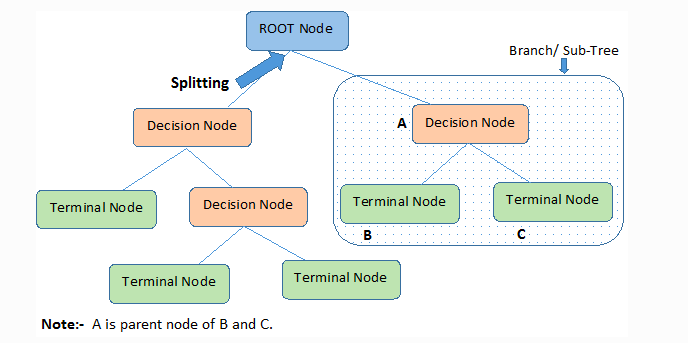
\includegraphics[width=0.6\textwidth]{figures/RandomForest.png}
    \caption{RandomForest Regressor}
    \label{fig:RandomForesy}
\end{figure}

\subsection{Model Characteristics and Suitability}
Random Forest Regressors offer several advantages that make them well suited for this application. First, they naturally capture nonlinear interactions between input parameters without requiring explicit feature engineering. Second, they are robust to noise and overfitting due to ensemble averaging. Third, they provide a strong baseline for comparison with more complex models such as artificial neural networks.

However, Random Forest models also exhibit certain limitations. Their prediction performance may degrade when extrapolating beyond the training data distribution, and their memory footprint increases with the number of trees. Despite these limitations, Random Forest Regressors serve as an effective and interpretable baseline surrogate model for evaluating the feasibility of data-driven thermal prediction in this thesis.


\newpage
\section{MLP-Sequence Model}

In addition to ensemble-based approaches, a neural network--based surrogate model is developed to capture complex nonlinear relationships between system inputs and thermal responses. Specifically, a Multi-Layer Perceptron (MLP) architecture is employed to learn the mapping between operating conditions and the reduced latent representation of time-dependent outputs obtained via Principal Component Analysis (PCA).

\subsection{Model Formulation}

The surrogate modeling problem is formulated as a supervised regression task:

\begin{equation}
f : \mathbb{R}^7 \rightarrow \mathbb{R}^5
\end{equation}

where the input vector $x \in \mathbb{R}^7$ represents the operating and boundary condition parameters, and the output corresponds to the 5-dimensional latent representation obtained from PCA.

The neural network approximates this mapping as a composition of nonlinear transformations:

\begin{equation}
\hat{y} = f_L(f_{L-1}(\dots f_2(f_1(x)) \dots))
\end{equation}

where each layer consists of an affine transformation followed by a nonlinear activation function.

\subsection{Network Architecture}

The MLP architecture consists of multiple fully connected layers designed to extract hierarchical feature representations.

\begin{itemize}
\item \textbf{Input layer:} 7 neurons (system input parameters)
\item \textbf{Hidden layers:} Fully connected layers with nonlinear activations
\item \textbf{Output layer:} 5 neurons (PCA coefficients)
\end{itemize}

Each hidden layer performs the transformation:

\begin{equation}
h^{(l)} = \phi \left( W^{(l)} h^{(l-1)} + b^{(l)} \right)
\end{equation}

where $W^{(l)}$ and $b^{(l)}$ denote the weights and biases of layer $l$, and $\phi(\cdot)$ is a nonlinear activation function.

In this work, the Rectified Linear Unit (ReLU) activation function is used:

\begin{equation}
\text{ReLU}(x) = \max(0, x)
\end{equation}

\subsection{Training Procedure}

The MLP model is trained using supervised learning by minimizing the Mean Squared Error (MSE) loss:

\begin{equation}
L = \frac{1}{N} \sum_{i=1}^{N} | y_i - \hat{y}_i |^2
\end{equation}

where $y_i$ represents the ground truth latent variables and $\hat{y}_i$ denotes the predicted outputs.

Model parameters are optimized using gradient-based optimization algorithms such as the Adam optimizer.

The training pipeline consists of the following steps:

\begin{enumerate}
\item Generate input samples using Latin Hypercube Sampling (LHS)
\item Run Dymola simulations to obtain time-series outputs
\item Apply PCA to reduce dimensionality (1800 $\rightarrow$ 5)
\item Construct supervised training pairs $(x, y_{\text{latent}})$
\item Train the MLP model
\end{enumerate}

\subsection{Reconstruction of Temporal Outputs}

After training, the MLP predicts latent PCA coefficients for unseen inputs. The original time-series outputs are reconstructed using the inverse PCA transformation:

\begin{equation}
\hat{y}*{\text{time}} = \text{PCA}^{-1}(\hat{y}*{\text{latent}})
\end{equation}

This enables efficient recovery of full temporal signals while maintaining low computational cost.

\subsection{Model Characteristics and Advantages}

Compared to Random Forest models, the MLP provides:

\begin{itemize}
\item Strong capability to model nonlinear relationships
\item Improved scalability with larger datasets
\item Compact parameter representation
\item Better generalization in high-dimensional spaces
\end{itemize}

\subsection{Limitations}

Despite its advantages, the current MLP formulation operates on a reduced latent representation and does not explicitly model temporal dependencies. The reconstruction of time-series outputs relies on PCA, which assumes linear relationships in the latent space.

Future work may include sequence-based architectures such as Recurrent Neural Networks (RNNs) or Transformer-based models to directly capture temporal dynamics.

